\begin{mybilan}
	\twoCol{
	
	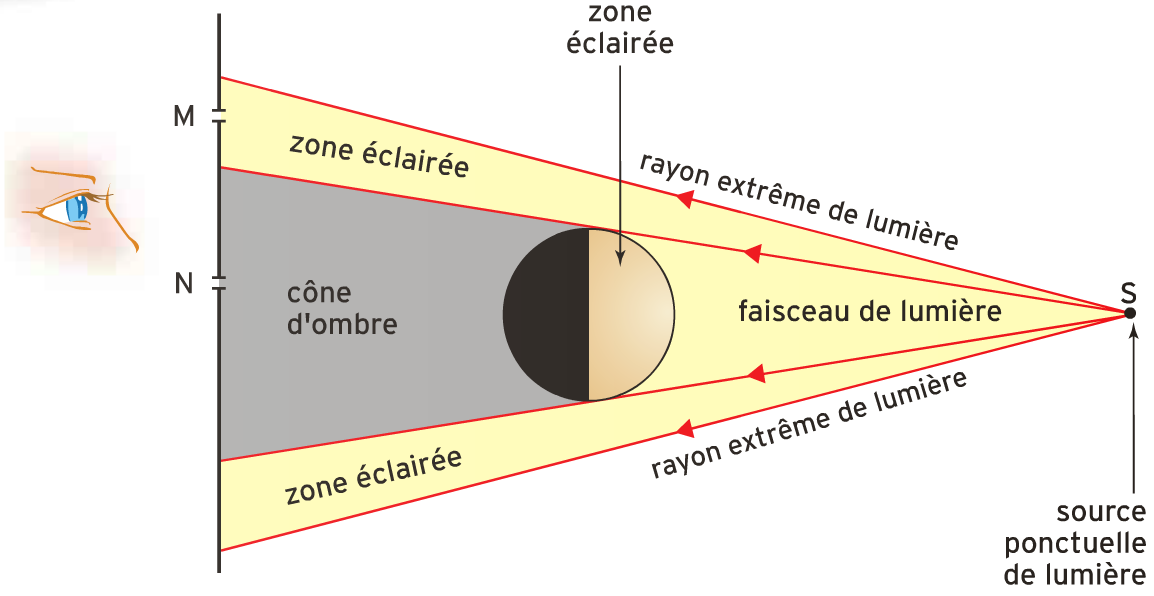
\includegraphics[scale=0.33]{bilan3}
	
	\begin{itemize}
		\item Lorsqu'un objet est éclairé par une source ponctuelle, elle détermine sur cet objet une \kw{zone éclairée}.
		\item Entre l'écran et l'objet on distingue une \kw{zone d'ombre} depuis laquelle l'observateur ne voit pas la source : c'est le \kw{cône d'ombre}. La zone depuis laquelle on voit la source de lumière est la \kw{zone éclairée}.
	\end{itemize}
	
	}
	
\end{mybilan}